\subsection{Ejercicio 2}

La IDT se corresponde con un arreglo de tamaño 255 de idt_entry. Un idt_entry es un struct que representará cada gate dentro de la tabla indicando selector de segmento de código donde se almacena la ISR, offset en dicho segmento y atributos del descriptor (present gate, tipo de gate y dpl). 

\begin{lstlisting} [caption={Struct de las gates},label=gate-struct]
typedef struct str_idt_entry_fld {
    unsigned short offset_0_15;
    unsigned short segsel;
    unsigned short attr;
    unsigned short offset_16_31;
} __attribute__((__packed__, aligned (8))) idt_entry;
\end{lstlisting}

\begin{figure}[H]
    \centering
    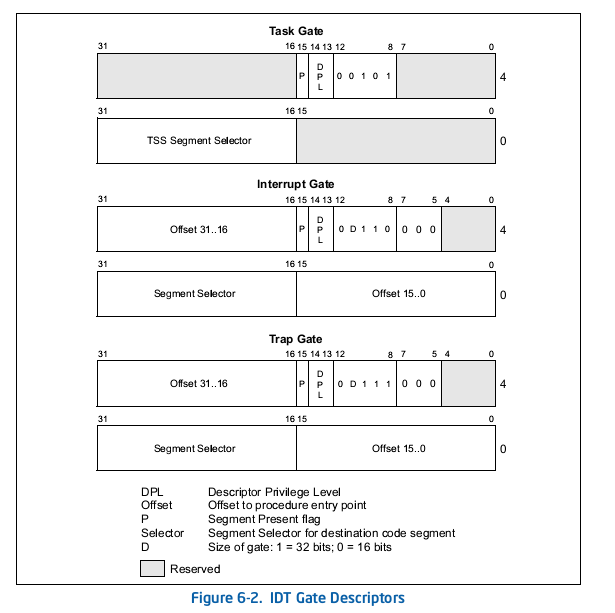
\includegraphics[width=\textwidth]{gates}
    \caption{Formato de las gates en IDT}
    \label{fig:gates}
\end{figure}



\subsubsection{Inicializar la IDT}

Para inicializar la IDT usamos una serie de macros tanto en C (para las gates) como en ASM (para las ISR) para facilitar la definición de las mismas.
De los macros generados usamos particularmente 3 de estos.
\begin{description}
\item [IDT_ENTRY_INTERRUPT] para las interrupciones de tipo 0-19, 32,33 y 40. Se setea con el descriptor de nuestro segmento flat de código de nivel 0, y offset (dividido de 0 a 15 y 16 a 31 bits por cuestiones de arquitectura) con puntero a una rutina genérica del 0-19, y específica para reloj (PIT y RTC) y teclado en interrupiones 32, 40 y 33 respectivamente. \\
Los atributos corresponden a nivel de privilegio 0, bit de present en 1 y tipo = 0xE $>>$ 2
\item [IDT_ENTRY_DEFAULT] para las interrupciones reservadas por Intel según manual (20-31) y aquellas "libres" para el usuario que no definimos (por lo tanto, no deberían ser accedidas durante la ejecución del sistema). \\
De esta forma podemos enterarnos, agregando un breakpoint en la rutina, si salta una interrupción que no estamos atendiendo.
\item [IDT_ENTRY_INTERRUPT_USER] para syscalls int 0x66 con privilegios de nivel usuario para llamar a SOY, DONDE y MAPEAR.
\end{description} 

Originalmente las interrupciones no-default se encargan de imprimir por pantalla su número de interrupción con un define que se hace dentro del macro de la isr.
\begin{lstlisting} [caption={Mensaje en el macro de isr},label=macro-msg]
% macro ISR 2
global _isr% 1

interrupt_msg_% 1 db         % 2
interrupt_msg_% 1_len equ    $ \$ $ - interrupt_msg_% 1

\end{lstlisting}

Todo esto quedó encapsulado en una función llamada idt_inicializar() que es ejecutada luego de cargar en IDTR un descriptor con la dirección donde se encuentra la IDT y su límite, empaquetados en el struct idt_descriptor de la cátedra.

